\documentclass[11pt]{article}

\usepackage[margin=1in]{geometry}
\usepackage{amsmath}
\usepackage{graphicx}
\usepackage{siunitx}
\usepackage[hidelinks]{hyperref}

\title{Frequency-Response Model for an Electromagnetic Seismometer}
\author{Zhicheng Gong, Jianing Pan}
\date{April 6, 2026}

\begin{document}

\maketitle

\section*{Purpose}
This note is a trial calculation of the relative frequency sensitivity of the seismometer. It is separate from the main report so that the model can be adjusted if we decide to refine the assumptions later.

\section*{Assumptions}
We use the observation that the mass-spring system oscillated about 50 times in 60 seconds, so the natural frequency is taken to be
\[
f_n \approx \frac{50}{60} \approx \SI{0.83}{\hertz}.
\]
The damping ratio was not measured directly, so this trial model uses $\zeta = 0.05$ as a reasonable small-damping estimate.

The mechanical part is modeled as a base-excited mass-spring-damper system. If the ground displacement is a sinusoid of fixed amplitude $Y$, then the relative displacement between magnet and coil is
\[
\left| \frac{Z}{Y} \right|
= \frac{r^2}{\sqrt{(1-r^2)^2 + (2 \zeta r)^2}},
\qquad
r = \frac{f}{f_n}.
\]
Since the coil voltage is proportional to the relative velocity of the magnet and coil, the mechanical sensitivity scales as
\[
|H_{\text{mech}}(f)| \propto 2 \pi f \left| \frac{Z}{Y} \right|.
\]

The acquisition chain includes:
\begin{enumerate}
  \item the analog op-amp feedback network, approximated as a low-pass stage with
  \[
  f_c \approx \frac{1}{2 \pi R C}
  = \frac{1}{2 \pi (866 \times 10^3)(330 \times 10^{-12})}
  \approx \SI{557}{\hertz},
  \]
  which is effectively flat over the low-frequency seismic band;
  \item the Arduino oversampling and 2048-sample averaging stage, which introduces a sinc-like low-pass response with first zero near \SI{4.70}{\hertz};
  \item the digital denoising FIR in \texttt{nerdaqII};
  \item the digital detrending high-pass filter with cutoff near \SI{0.033}{\hertz};
  \item the long-period boost filter used by the code.
\end{enumerate}

\section*{Result}
Figure~\ref{fig:sensitivity-model} shows the normalized response of the mechanical stage, the acquisition chain, and the combined response. In this trial model the total sensitivity peaks at about \SI{0.84}{\hertz}, very close to the estimated natural frequency. By \SI{2.5}{\hertz}, the combined sensitivity has already dropped to roughly $2 \times 10^{-3}$ of its peak value, so the full system strongly favors slow oscillations and impulsive low-frequency motion over faster vibration.

\begin{figure}[h]
  \centering
  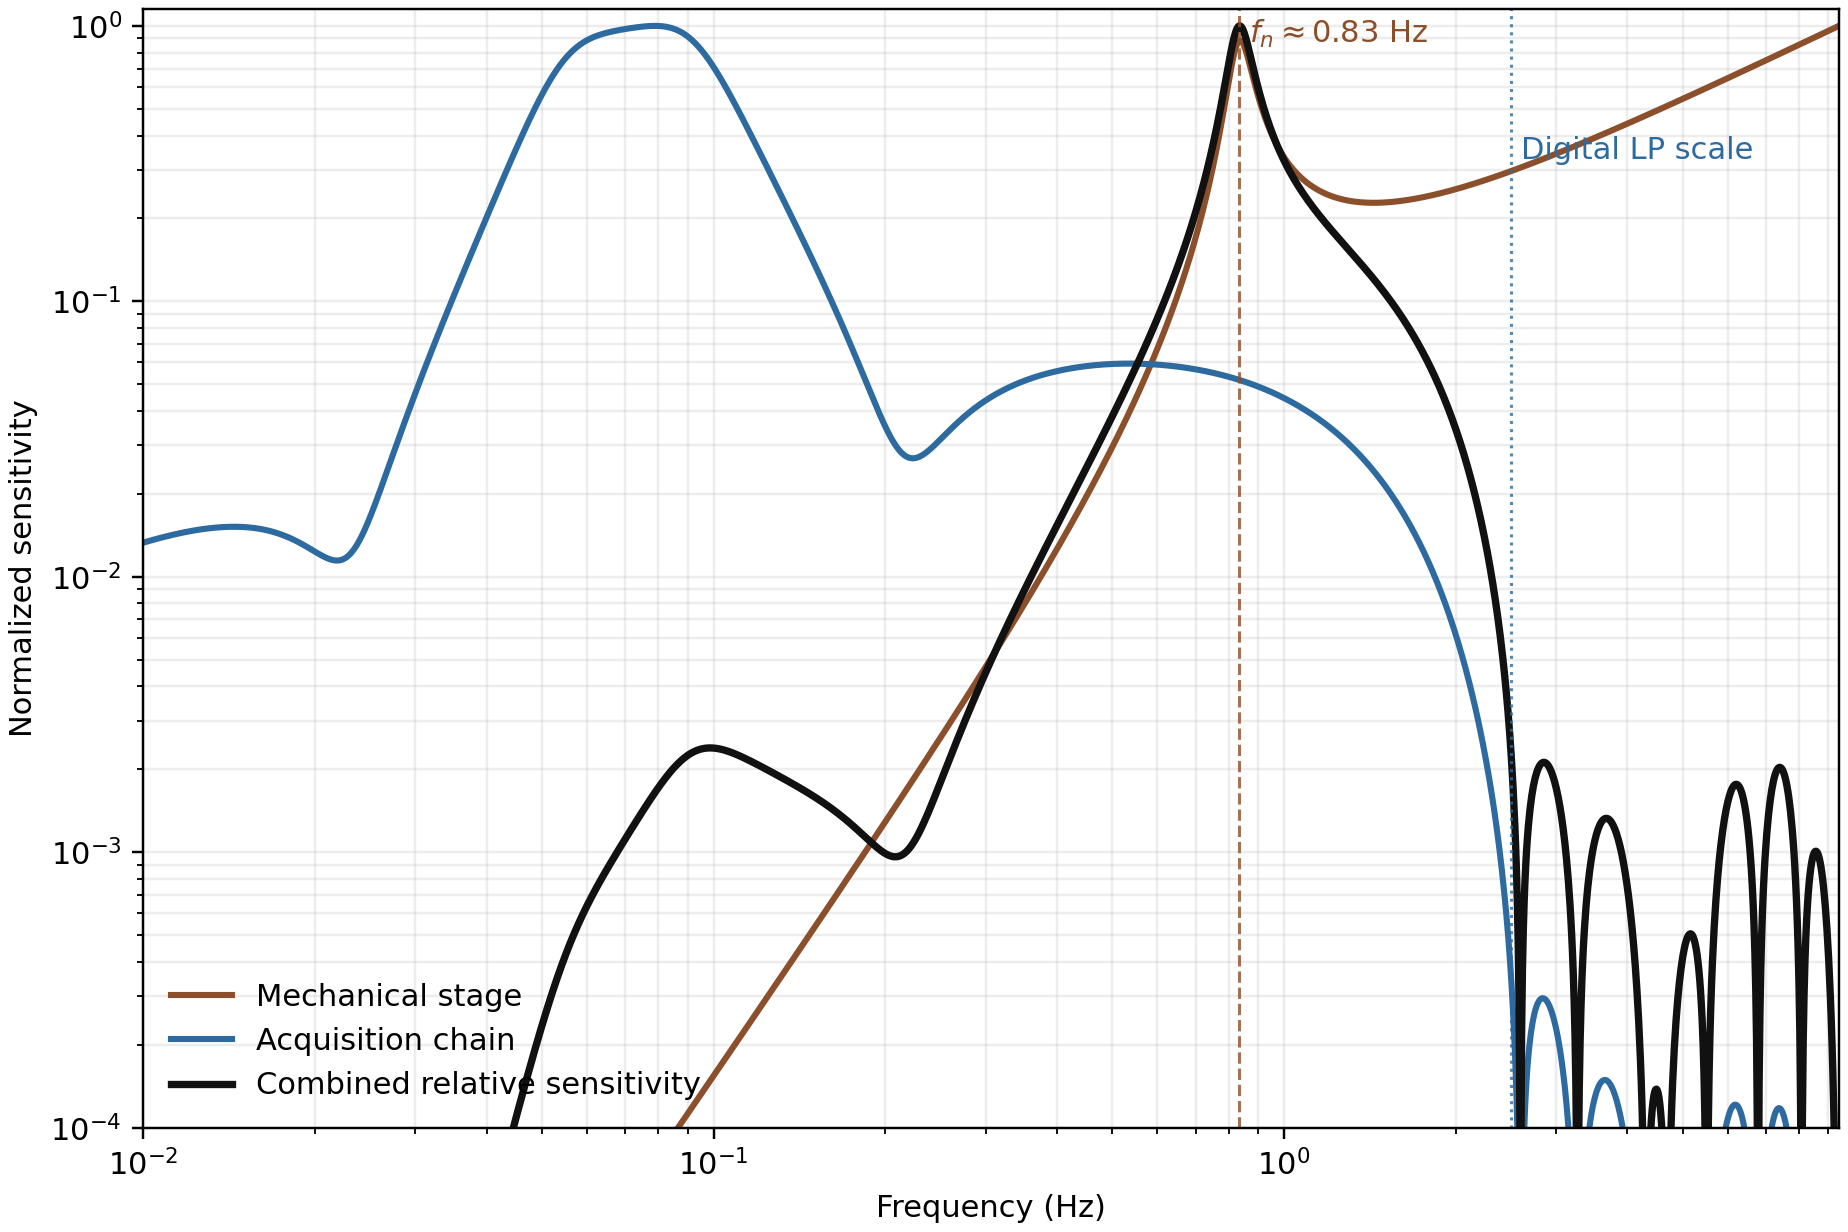
\includegraphics[width=0.9\linewidth]{images/sensitivity_model.png}
  \caption{Trial normalized sensitivity model for the seismometer. The black curve is the combined response of the mass-spring stage and the acquisition chain.}
  \label{fig:sensitivity-model}
\end{figure}

Figure~\ref{fig:modes-model} compares two practically important \texttt{nerdaqII} choices using the same mechanical model. Mode 1 corresponds to oversampled ADC output only, while Mode 4 is the default path that adds the FIR denoising filter, the detrending high-pass filter, and the long-period boost. The curves are normalized separately, so the comparison shows how the default processing reshapes frequency preference rather than absolute output amplitude.

\begin{figure}[h]
  \centering
  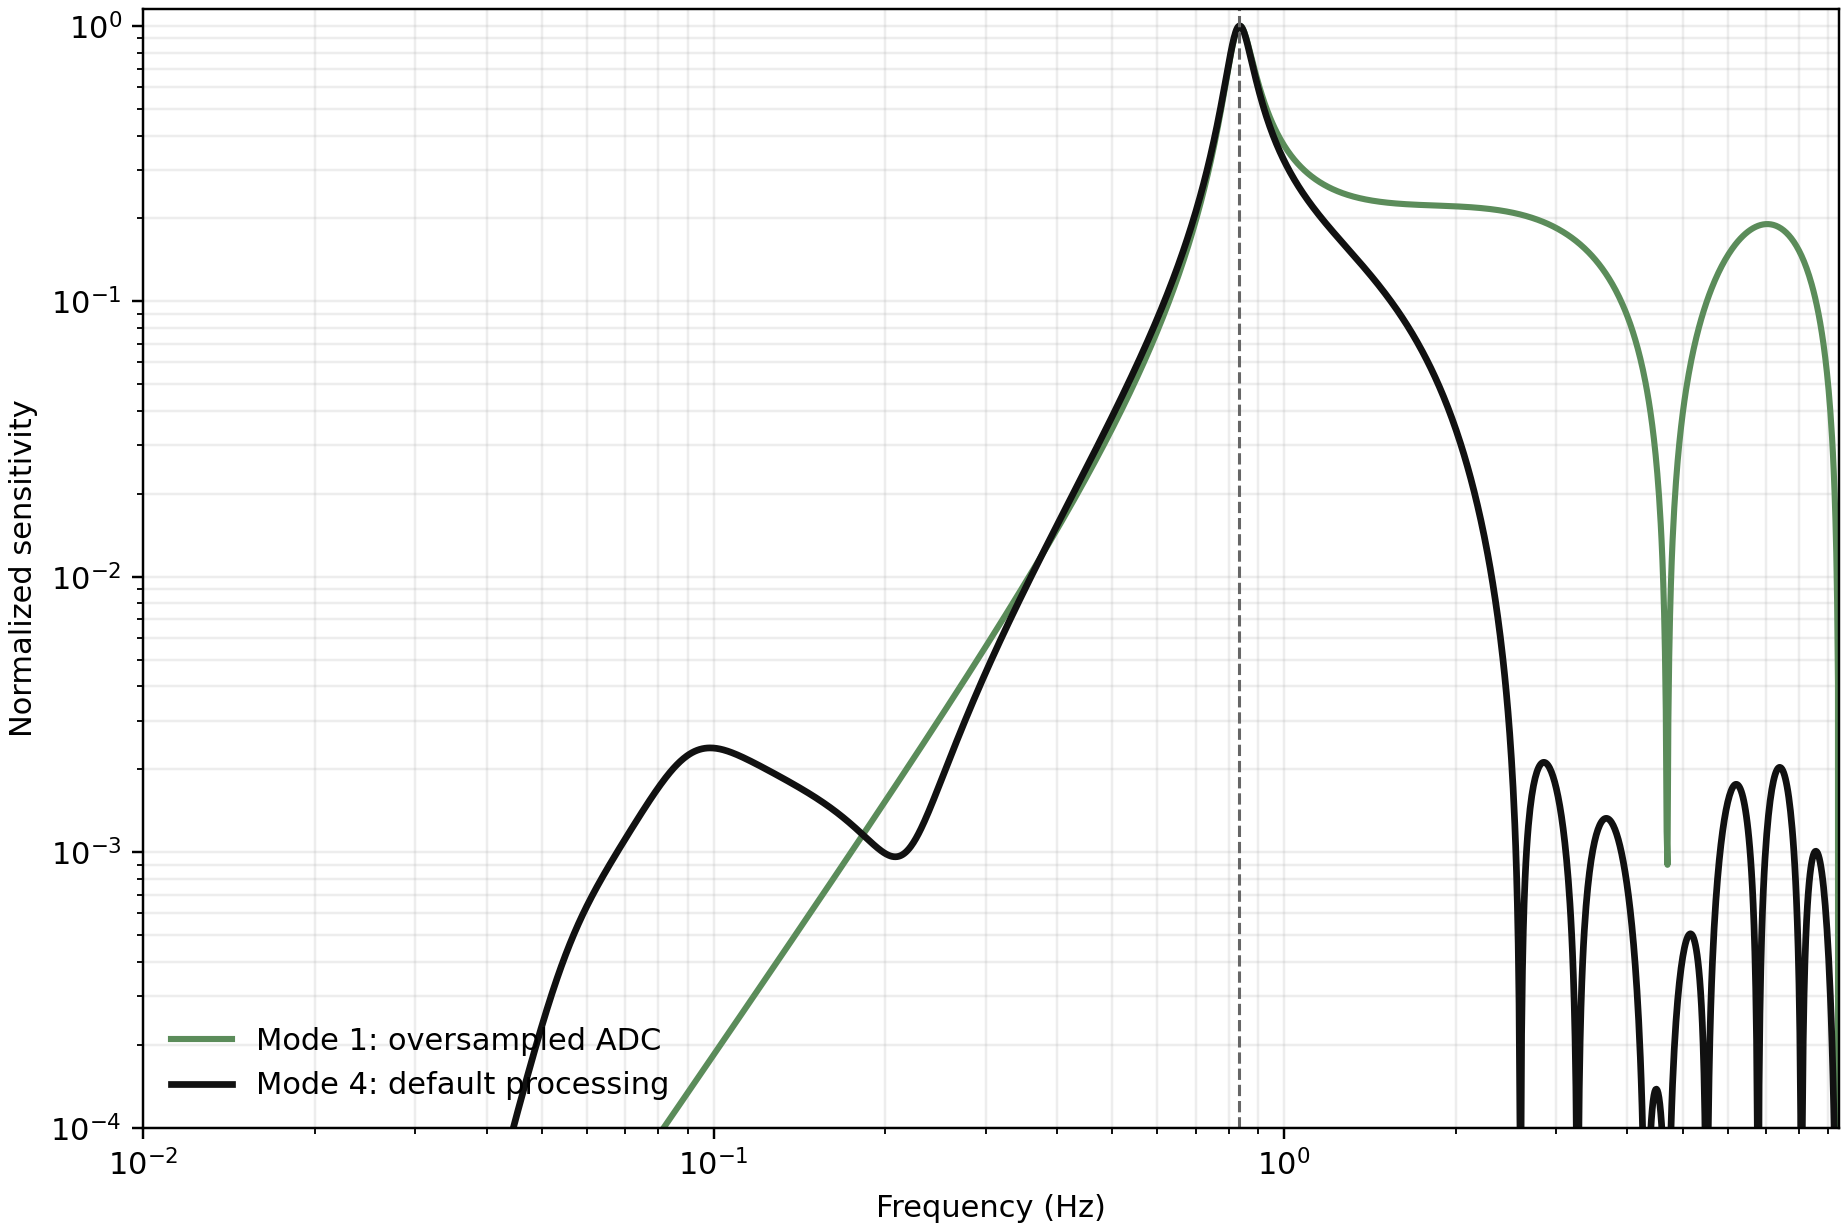
\includegraphics[width=0.9\linewidth]{images/sensitivity_modes_comparison.png}
  \caption{Relative sensitivity predicted for a minimally processed path (Mode 1) and the default \texttt{nerdaqII} path (Mode 4). The default mode is more selective and more strongly shaped toward the intended low-frequency seismic band.}
  \label{fig:modes-model}
\end{figure}

\section*{Interpretation}
This model is qualitatively consistent with the experiments. The strongest response occurs close to the mass-spring resonance, while the digital filtering suppresses higher-frequency components. That agrees with the observation that the instrument responded well to jumping, running, high heels, and other sudden low-frequency disturbances, but was much less sensitive to quiet walking or smoother motion. The mode comparison also makes clear that the default \texttt{nerdaqII} settings are not neutral: they increase interpretability for seismic-style signals, but they also make the recorded trace less representative of the raw coil output.

This plot should be interpreted as a \emph{relative} sensitivity curve rather than an absolute calibration. The true response would depend on the actual damping ratio, the coil constant, the source impedance of the coil, and whether one compares equal displacement, equal velocity, or equal acceleration input at different frequencies.

\end{document}
